\section{Building and Flying Two Hexacopters}

After finishing a master thesis~\cite{joshua_master_thesis} wherein I developed an algorithm for autonomously landing a drone using
fiducial markers in simulation, the next step was to test this method on physical platforms.
The algorithm required identifying fiducial markers through image analysis,
tracking the markers via a gimbal-mounted camera,
calculating position targets in order to direct the drone towards the landing pad,
and communicating those position targets to the flight control software.
The base frame for the drones are the Tarot 680 hexacopter kit, which provides a good thrust-to-weight ratio,
good flight stability,
and space for mounting multiple computational components.
A combination of Raspberry Pi and Navio2~\cite{navio2_website} shield serve as a flight controller
which can communicate with a companion board.
The companion boards (a Google Coral Dev board and an NVIDIA Jetson Nano) communicate via a USB network to the flight
controller and perform all heavy computations involving image analysis, coordinate system transforms, PID control,
and position target generation.

An overview the components is as follows:

\begin{itemize}
    \item \textbf{11.1 V LiPo Battery:} this battery provides power to a battery eliminator circuit (BEC) for isolation of the power system for the computational electronics (the flight controller and companion board).
    \item \textbf{BEC (Battery Eliminator Circuit):} the BEC transforms 11.1V power to 5V power for the flight controller and companion board. The flight controller and companion board each have their own 4A channel to meet their given power requirements.
    \item \textbf{Flight Controller:} this combination of a Raspberry Pi 3 B+ and Navio2 shield runs the ArduPilot software to control the drone, and communicates with the companion board to control the gimbal.
    \item \textbf{Telemetry Radio:} the telemetry radio provides two-way communication between the flight controller and a ground control station that is also fitted with its own telemetry radio. It is connected to the flight controller via USB. The software on the ground control station provides an interface for real-time status messages and sending high-level commands.
    \item \textbf{RC Receiver:} the RC receiver provides a one-way radio link between the pilot's transmitter and the flight controller, allowing the pilot to manually control the drone. It is connected to the flight controller via SBus which provides an 8-channel multiplexed PWM signal to reduce the needed wires and space. This provides an interface for control by a human pilot, which is often used in testing but will eventually be mostly unused.
    \item \textbf{22.2 V LiPo Battery:} this battery provides power to the speed controllers and gimbal.
    \item \textbf{Speed Controllers:} the speed controllers receive a PWM signal from the flight controller which indicates a throttle value. They then provide corresponding power signals to the motors.
    \item \textbf{Motors:} the motors spin propellers to provide thrust in order to control the drone's position in the air.
    \item \textbf{Gimbal:} the gimbal controls the orientation of the camera based on PWM signals from the flight controller which indicate target angles. Its onboard IMU and driver filter the motion of the camera in order to provide a smooth camera image.
    \item \textbf{Companion Board:} the companion board reads an image from the camera and calculates the position of the landing pad relative to the drone. It then communicates this information to the flight controller via an Ethernet over USB connection using ROS.

\end{itemize}

\begin{figure}
    \centering
    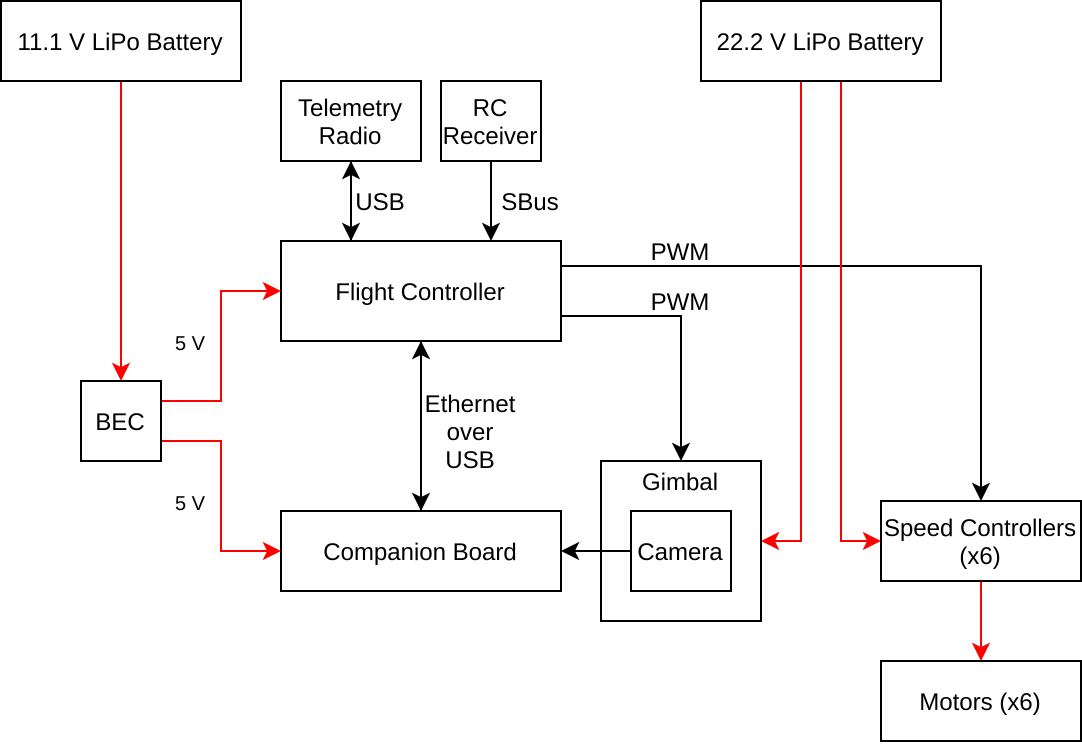
\includegraphics[width=0.8\textwidth]{images/hardware.png}
    \caption{Hardware Setup}
    \label{fig:hardware_setup}
\end{figure}

The computational components require some protection from the harsh Icelandic weather,
and we therefore designed and 3D-printed a component mounting plate with a connector for a canopy.
We also designed and printed cases to protect camera modules and allow them to be mounted in a gimbal with a GoPro form factor.
The final versions of these components (after several iterations) can be seen in Figure \ref{figure:printed_parts}.
The fully assembled hexacopters are shown in Figure \ref{figure:drone_pictures}

\begin{figure}
  \centering
  \begin{subfigure}[b]{0.33\textwidth}
    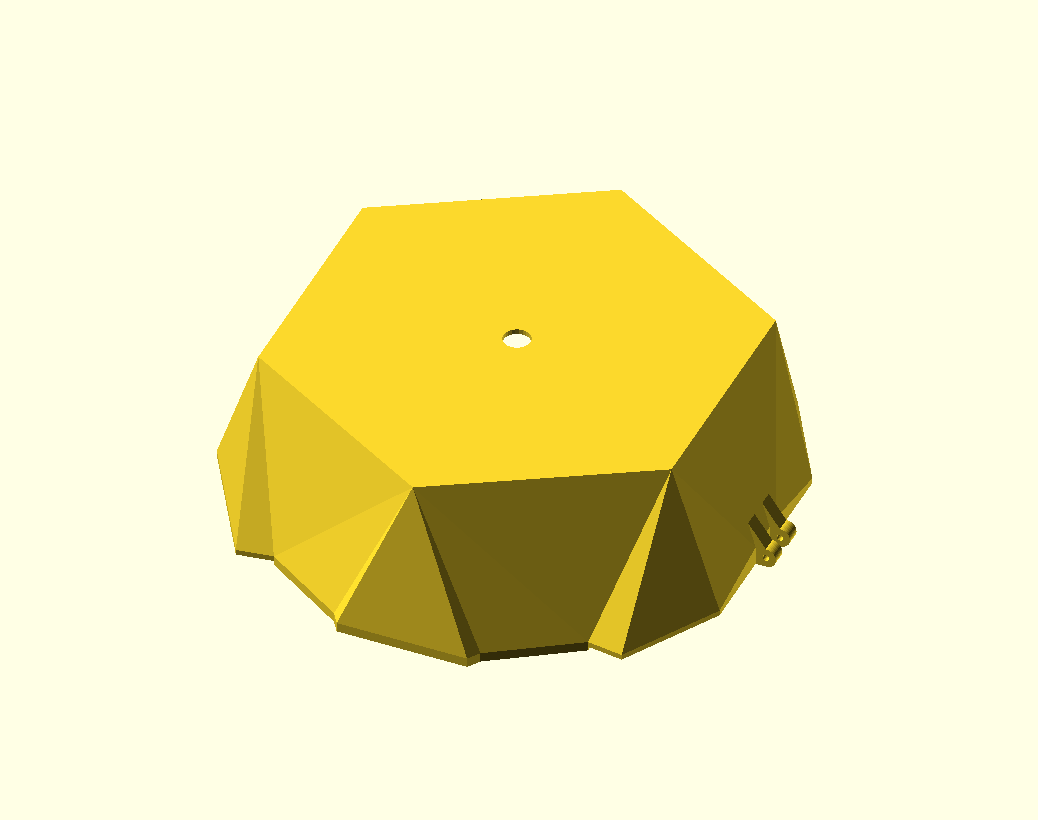
\includegraphics[width=\textwidth]{canopy.png}
    \caption*{Protective Canopy.}
  \end{subfigure}
  \hspace{1cm}
  \begin{subfigure}[b]{0.33\textwidth}
    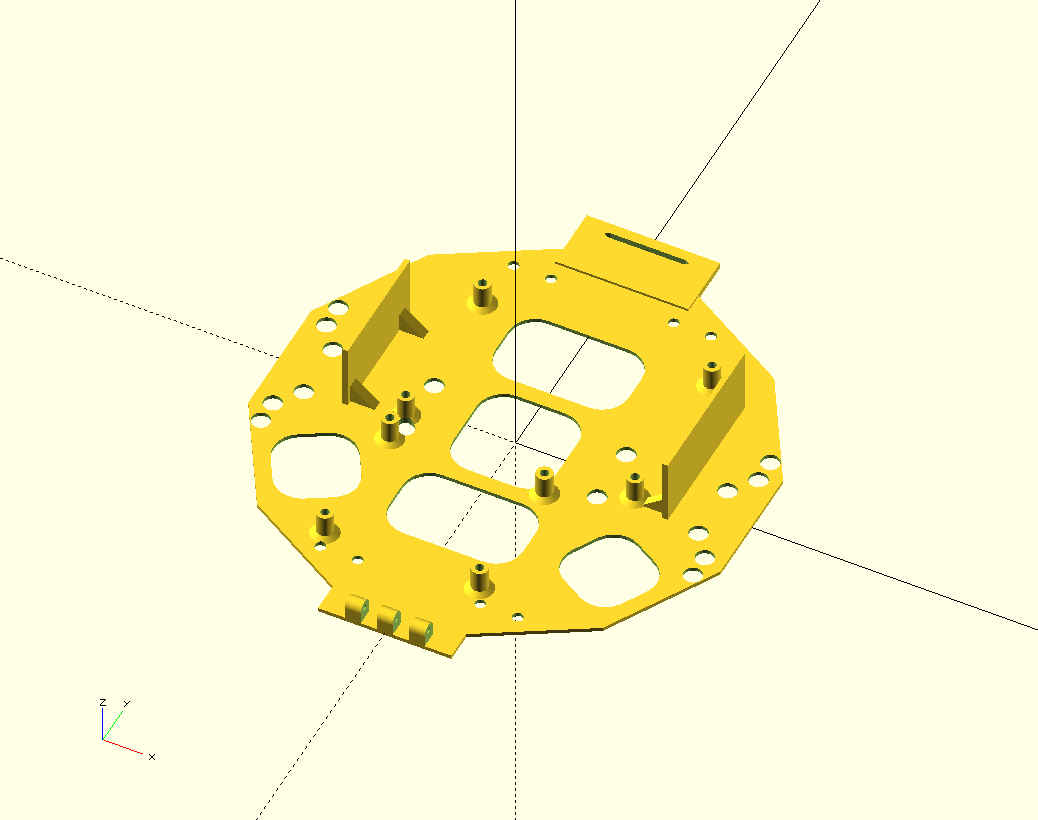
\includegraphics[width=\textwidth]{component_mounting_plate.png}
    \caption*{Component mounting plate.}
  \end{subfigure}

  \begin{subfigure}[b]{0.33\textwidth}
    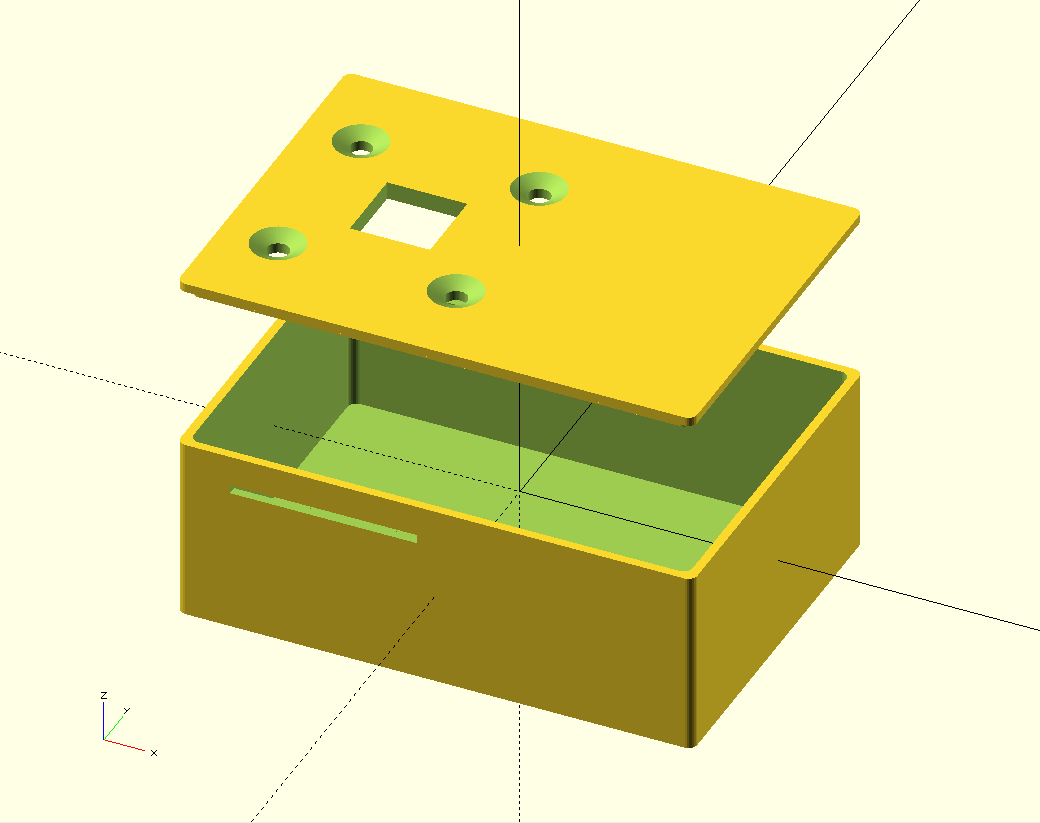
\includegraphics[width=\textwidth]{coral_case.png}
    \caption*{Google Coral camera case.}
  \end{subfigure}
  \hspace{1cm}
  \begin{subfigure}[b]{0.33\textwidth}
    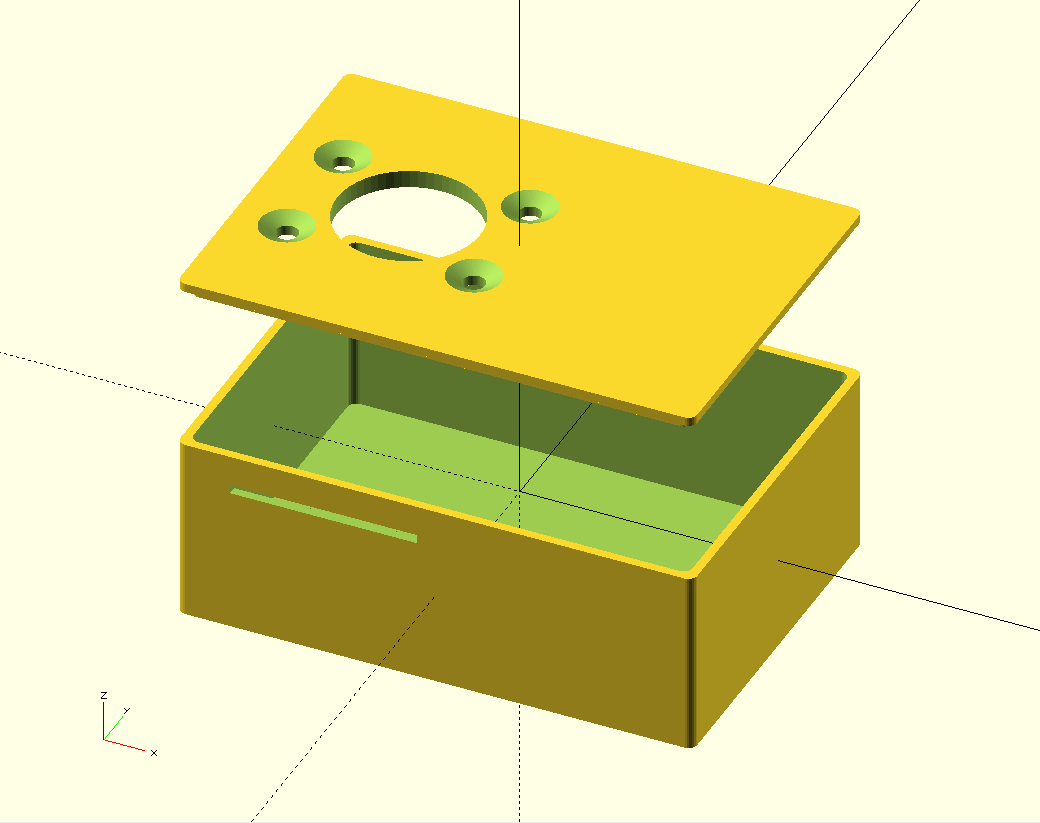
\includegraphics[width=\textwidth]{nano_case.png}
    \caption*{Jetson Nano camera case.}
  \end{subfigure}
  \caption{3D printed parts for the Tarot hexacopters.}
  \label{figure:printed_parts}
\end{figure}

\begin{figure}
    \begin{subfigure}[b]{0.48\textwidth}
        \centering
        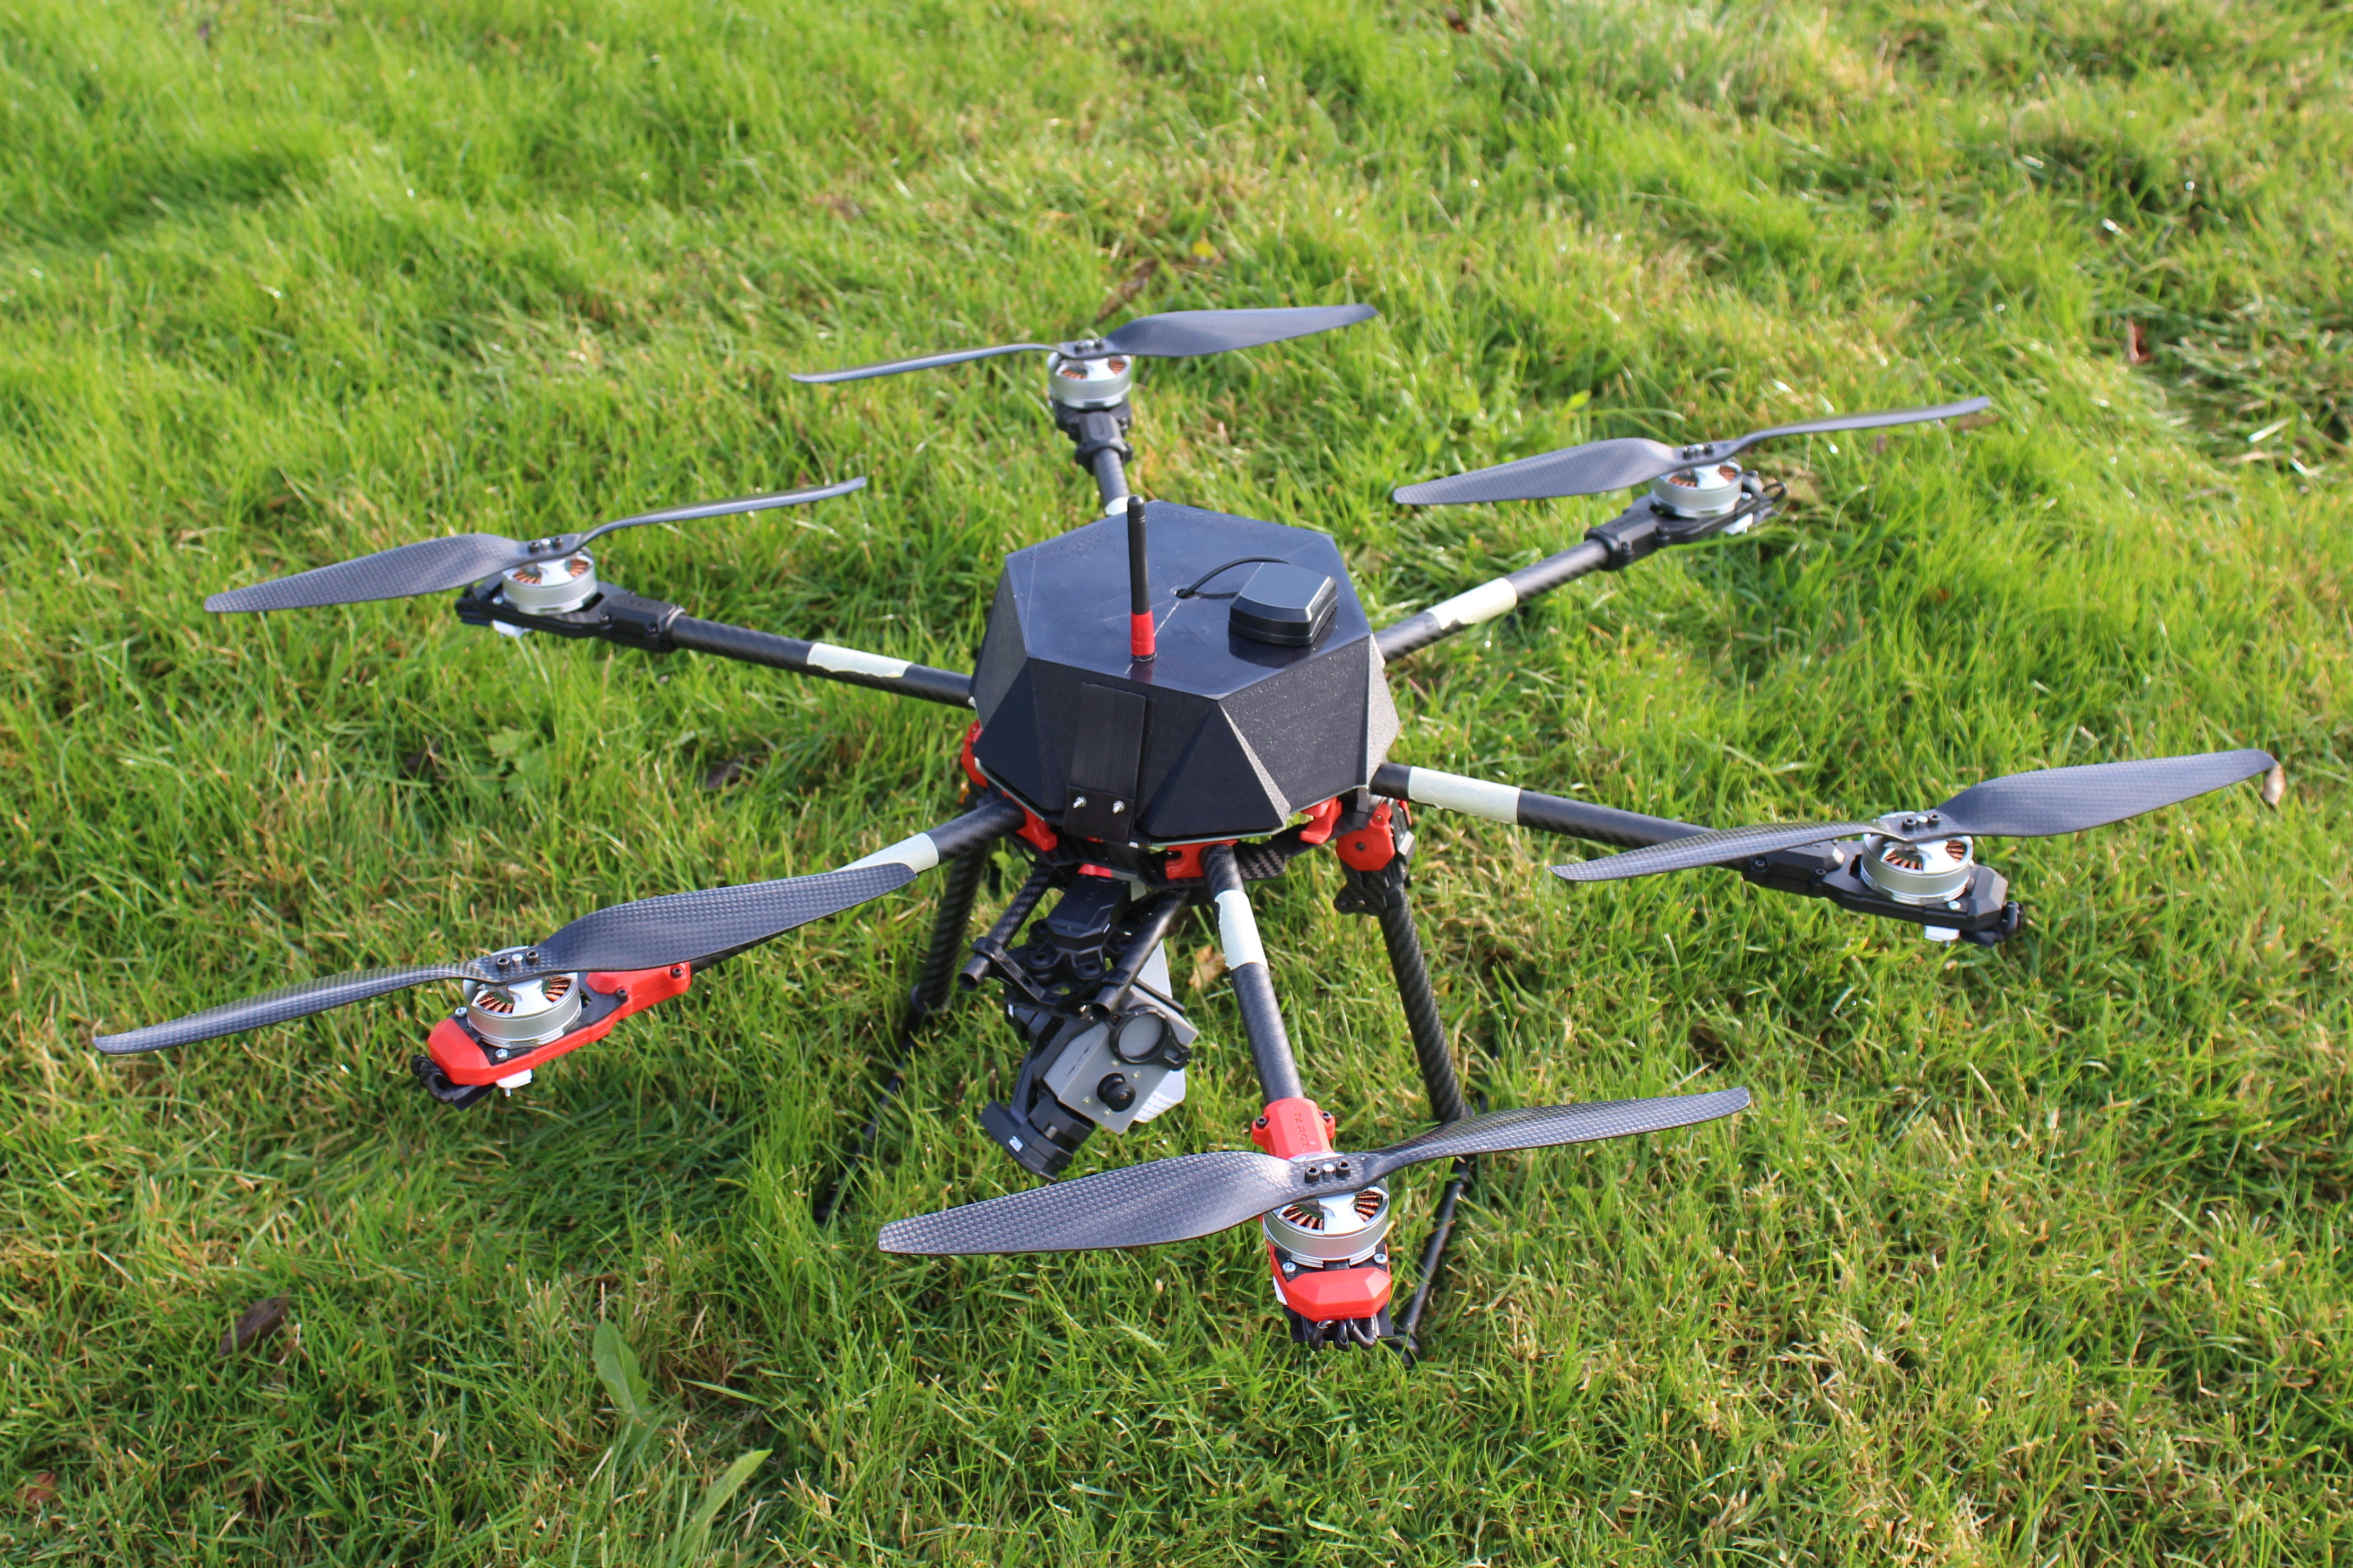
\includegraphics[width=\textwidth]{images/jetson_drone.JPG}
        \caption{The Jetson drone.}
        \label{fig:jetson_drone}
    \end{subfigure}
    \begin{subfigure}[b]{0.48\textwidth}
        \centering
        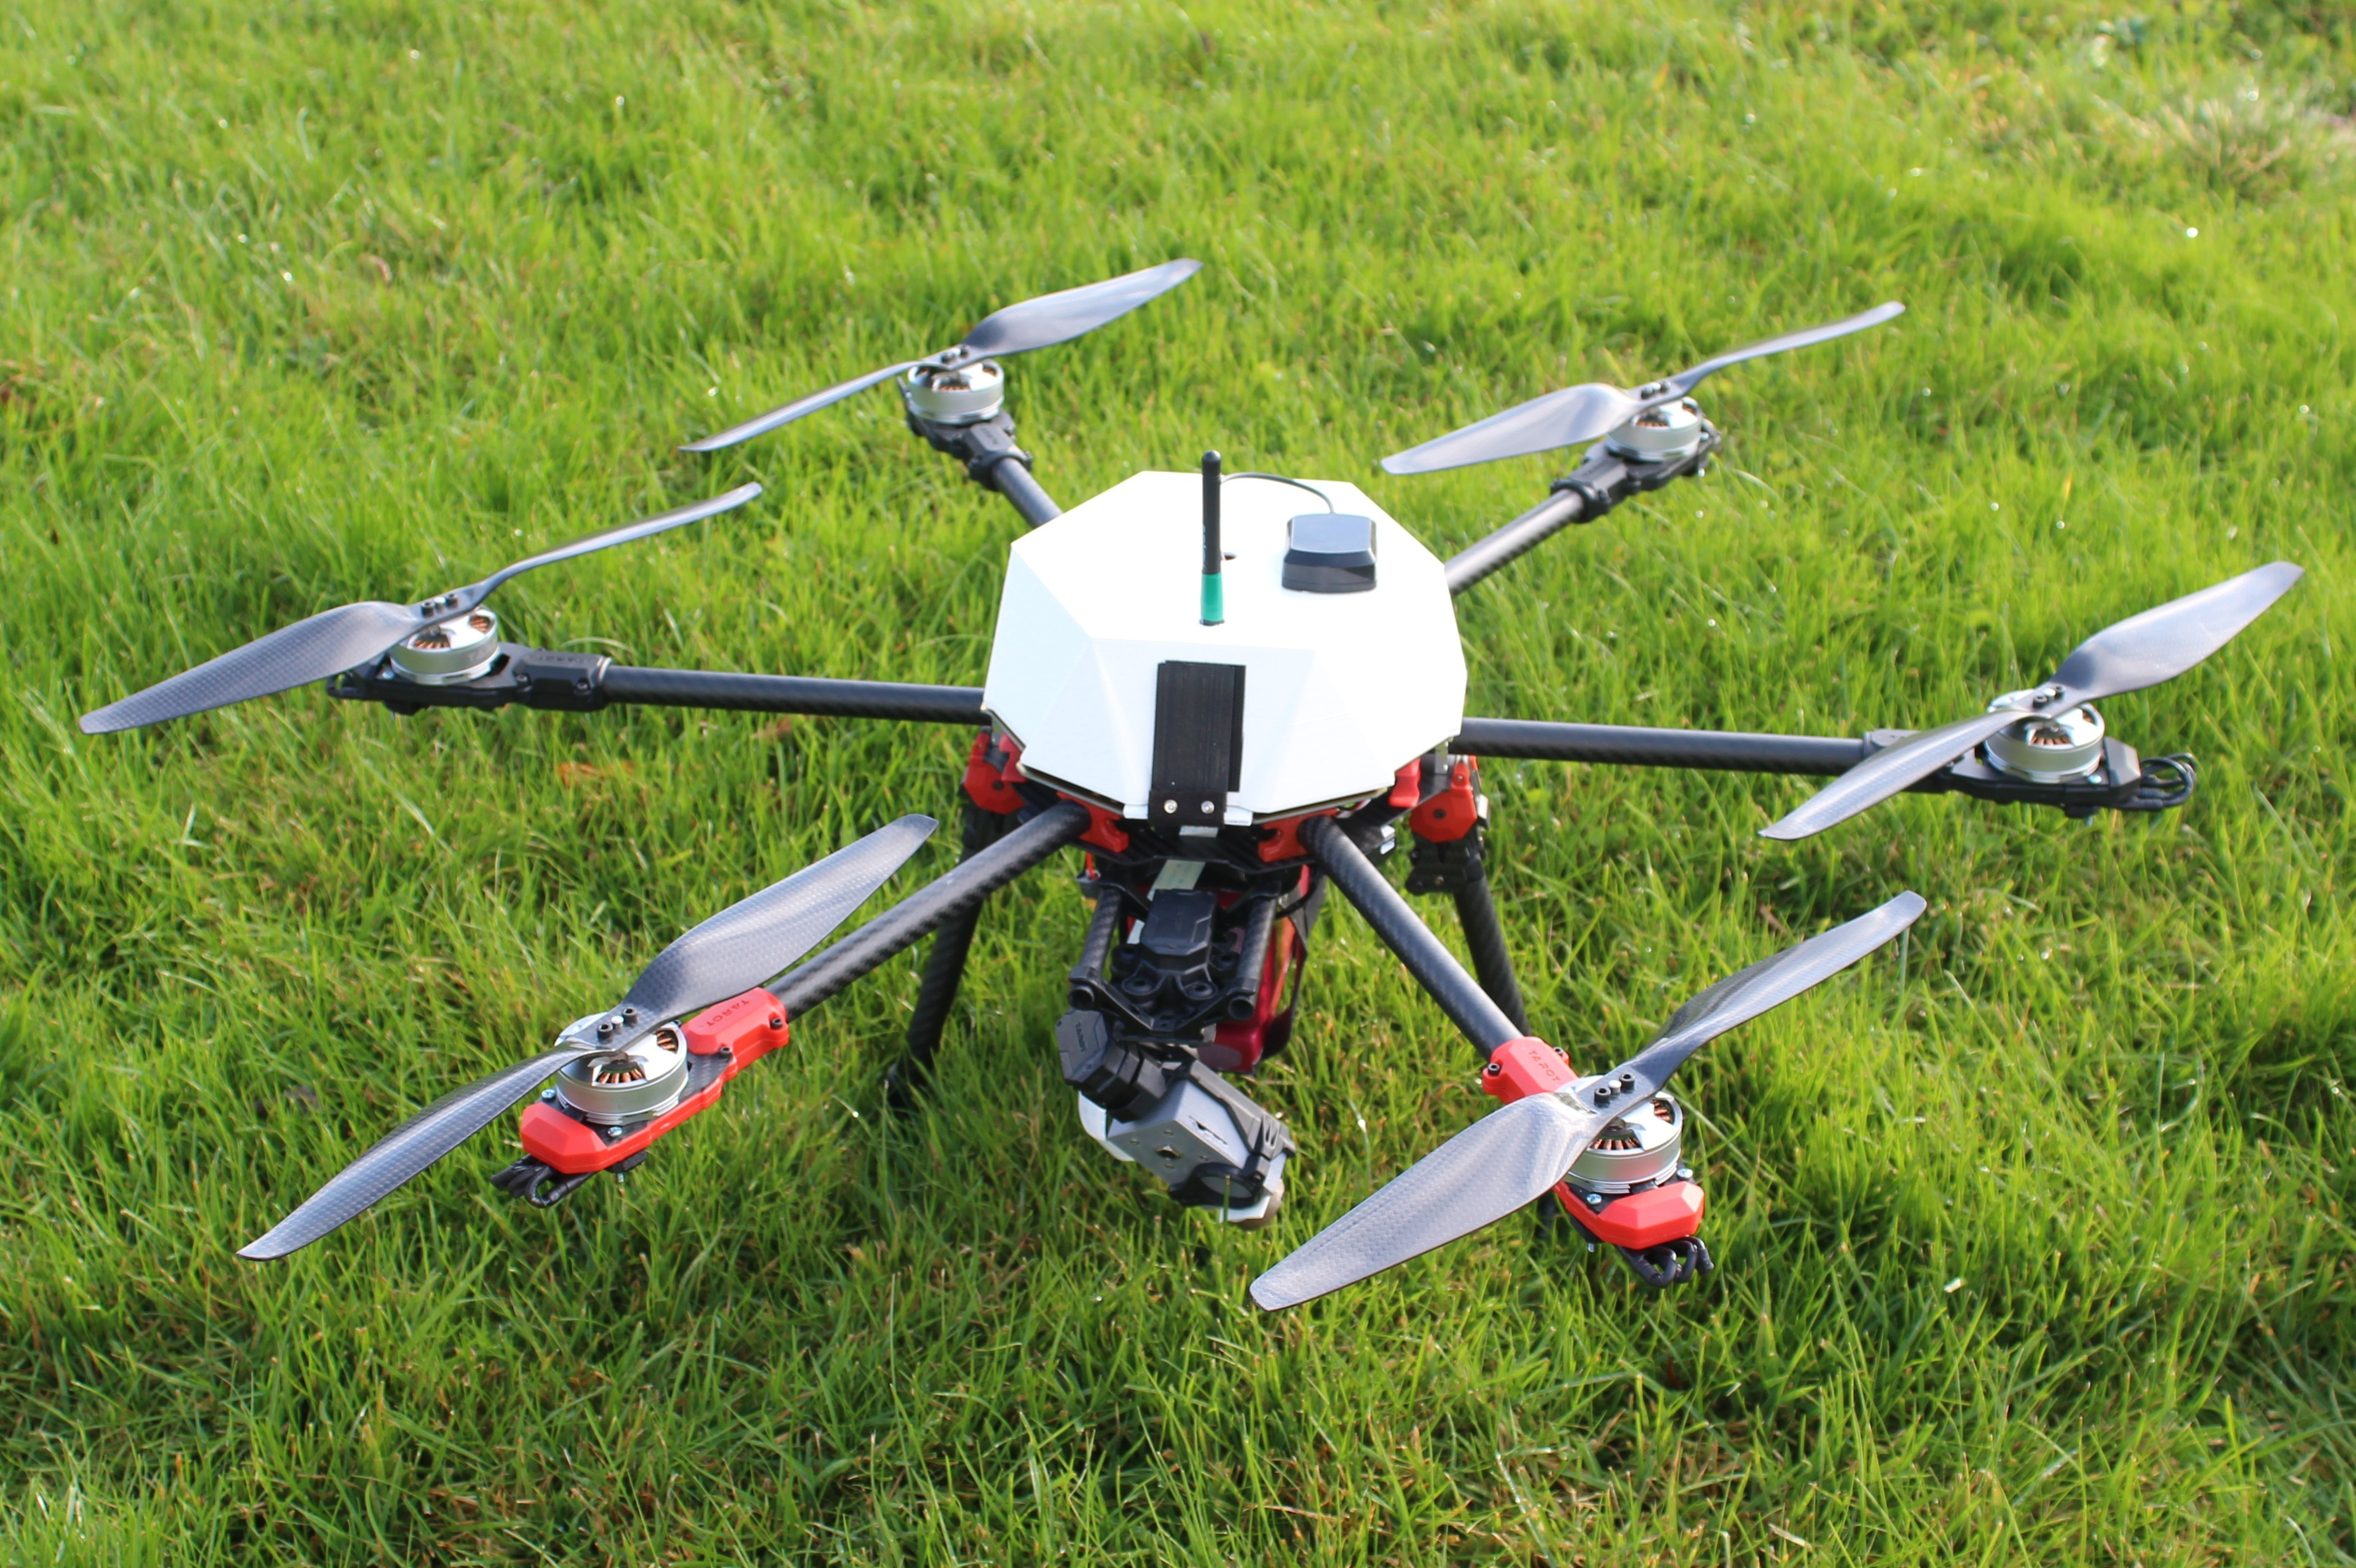
\includegraphics[width=\textwidth]{images/coral_drone.JPG}
        \caption{The Coral drone.}
        \label{fig:coral_drone}
    \end{subfigure}

    \begin{subfigure}[b]{0.48\textwidth}
        \centering
        \includegraphics[width=\textwidth]{images/jetson_electronics.JPG}
        \caption{The Jetson drone's electronics compartment.}
        \label{fig:jetson_electronics}
    \end{subfigure}
    \begin{subfigure}[b]{0.48\textwidth}
        \centering
        \includegraphics[width=\textwidth]{images/coral_electronics.JPG}
        \caption{The Coral drone's electronics compartment.}
        \label{fig:coral_electronics}
    \end{subfigure}

    \caption{The assembled drones and their electronics compartments.}
    \label{figure:drone_pictures}
\end{figure}

The algorithm is implemented as a set of ROS modules, as explained below:
\begin{enumerate}
    \item \texttt{gscam} retrieves camera input and makes it available as a ROS topic,
    \item \texttt{whycon\_ros} analyzes camera images to detect WhyCon/WhyCode markers and determine their pose,
    \item \texttt{gimbal\_controller} reads the poses of any detected markers,
                                      passes this information as input to two PID systems,
                                      converts the output of the PID systems to PWM outputs,
                                      and forwards the PWM outputs to the autopilot software to control the gimbal.
    \item \texttt{landing\_controller} reads the poses of any detected markers,
                                        performs coordinate system transforms to generate a target position,
                                        and forwards them to the autopilot software.
\end{enumerate}

\subsection{Results}

